\documentclass{standalone}

\usepackage[euler-digits]{eulervm}

\usepackage{tikz}
\tikzset{every node/.style={ellipse,align=center,draw,shade,minimum size=6mm,inner sep=0pt}}
\tikzset{every path/.style={->,>=latex}}
\tikzset{t/.style={rectangle}}
\tikzset{r/.style={top color=red}}
\tikzset{g/.style={top color=green}}
\tikzset{b/.style={top color=blue}}

\usetikzlibrary{shapes}

\begin{document}
    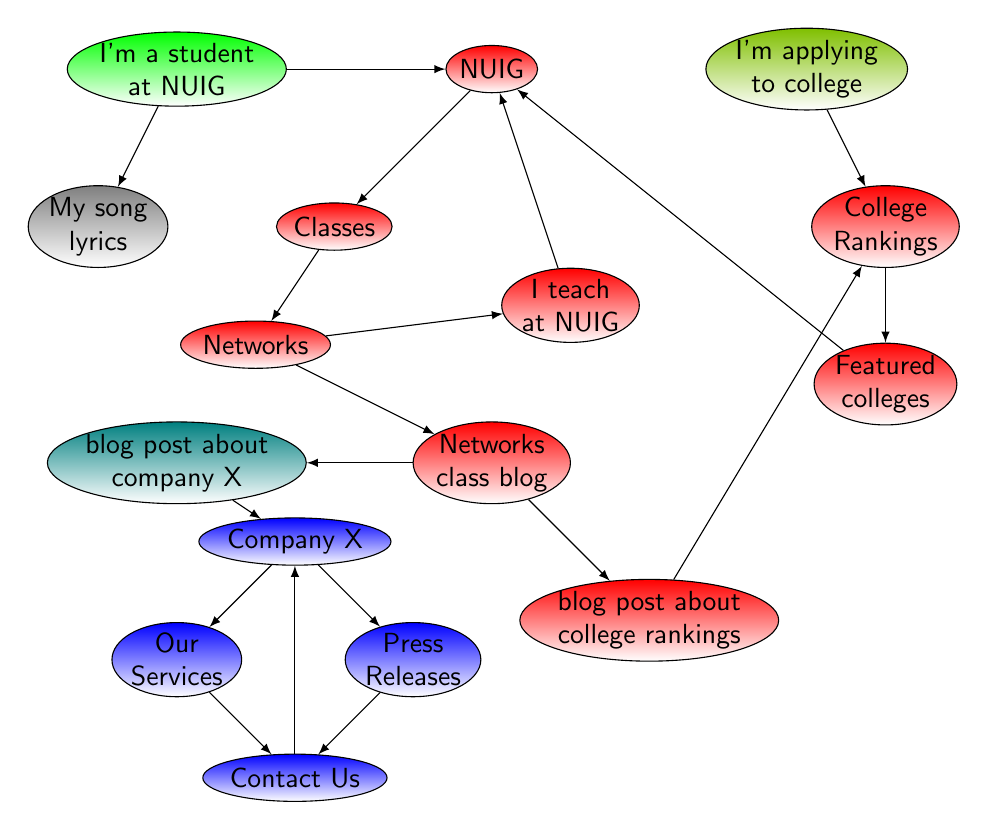
\begin{tikzpicture}[font=\sffamily]
\node[r](college) at (0,7) {NUIG};
\node[g](student) at (-4, 7) {I'm a student\\ at NUIG};
\node[top color=green!50!orange](apply) at (4, 7) {I'm applying\\ to college};
\node(lyrics) at (-5, 5) {My song \\lyrics};
\node[r](classes) at (-2,5) {Classes};
\node[r](networks) at (-3,3.5) {Networks};
\node[r](teacher) at (1,4) {I teach\\at NUIG};
\node[r](ranking) at (5,5) {College\\Rankings};
\node[r](feature) at (5,3) {Featured\\colleges};
\node[r](blog) at (0,2) {Networks\\class blog};
\node[r](post1) at (2,0) {blog post about\\college rankings};
\node[top color=blue!50!green](post2) at (-4,2) {blog post about\\company X};
\node[b](company) at (-2.5,1) {Company X};
\node[b](services) at (-4,-0.5) {Our\\Services};
\node[b](press) at (-1,-0.5) {Press\\Releases};
\node[b](contact) at (-2.5,-2) {Contact Us};

\draw (student) -- (college);
\draw (student) -- (lyrics);
\draw (college) -- (classes);
\draw (classes) -- (networks);
\draw (networks) -- (blog);
\draw (networks) -- (teacher);
\draw (teacher) -- (college);
\draw (blog) -- (post1);
\draw (blog) -- (post2);
\draw (apply) -- (ranking);
\draw (ranking) -- (feature);
\draw (feature) -- (college);
\draw (post1) -- (ranking);
\draw (post2) -- (company);
\draw (company) -- (services);
\draw (company) -- (press);
\draw (services) -- (contact);
\draw (press) -- (contact);
\draw (contact) -- (company);
    \end{tikzpicture}
\end{document}
